\section{Test Cases}
The training cases are not truly representative of an array where both hybridisation partners have the same CNV. Cy3 and Cy5 dyes are incorporated with varying efficacy so the reference value will vary. When calculating the Z score for the training set comparing the signal intensity of one dye to the reference value of the other dye may introduce error.
\paragraph*{}
The same thresholds were applied to 69 test cases (Table \ref{tab:testcasetable}). 



\subsection{A greater sensitivity was seen using more representative feature extraction files}
There was 100\% sensitivity using a Z score below 4 and there were no false positive calls using a Z score above 3.55 (Table \ref{tab:testcasetable}). 


\begin{table}[h]
\centering
\caption[Test cases: Calls made at a range of thresholds]{Test cases: A call was made in the expected CNV region in all cases with a threshold below 4. There were no false positive calls made with a threshold above 3.55}
\label{tab:testcasetable}
\resizebox{\textwidth}{!}{%
\begin{tabular}{@{}lccccccc@{}}
\cmidrule(l){2-8}
\multirow{2}{*}{}                    & \multicolumn{7}{c}{Z score}                                               \\ \cmidrule(l){2-8} 
                                     & 2.375    & 3        & 3.5      & 3.55     & 3.75     & 4        & 4.25    \\ \cmidrule(l){2-8} 
\% True Positive arrays (n)          & 100 (69) & 100 (69) & 100 (69) & 100 (69) & 100 (69) & 100 (69) & 97 (67) \\
\% Arrays with false positives (n)   & 13 (9)   & 8.7 (6)  & 1.4 (1)  & 0        & 0        & 0        & 0       \\
Number of false positive calls (max) & 48 (28)  & 9 (3)    & 1 (1)    & 0        & 0        & 0        & 0      
\end{tabular}%
}
\end{table}

\subsection{Suitability of reference range}
There were no recurring false positive calls.

\subsection{Proportion of CNV regions covered by calls}
As shown in Figure \ref{fig:testcasestrueposcoverage} with the exception of 8 arrays with the 750 probe deletion on chromosome 22 (Table \ref{tab:testset_calls}) at least 25\% and on average 66\% of the probes within the known CNV were within a call. Cases with the chromosome 22 deletion is described in section \ref{ch:analysisof22del}

\begin{figure}[h]
\centering
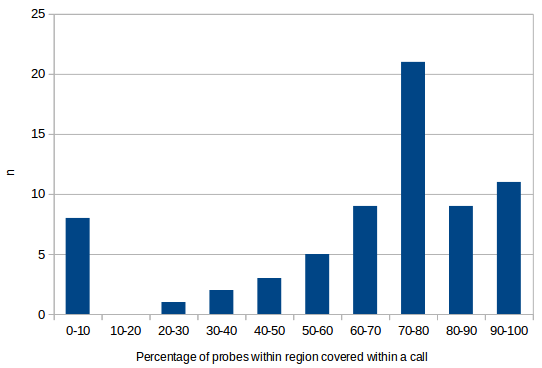
\includegraphics[width=1\linewidth]{./Figures/testcasestrueposcoverage}
\caption[Test cases: the proportion of probes within reported CNV included by a call at a threshold of 3.55]{The proportion of probes within reported CNV included by a call at a threshold of 3.55.}
\label{fig:testcasestrueposcoverage}
\end{figure}